% Presentación para Pronatura Noreste. Las cifras «entre comillas latinas» se llenan con informe/generar.py,
% que escribe presentacion.tex. Compilar:  python informe/generar.py && cd informe && tectonic presentacion.tex
\documentclass[aspectratio=169,10pt]{beamer}
\usepackage[spanish,es-noshorthands]{babel}
\unaccentedoperators
\usepackage{amsmath,amssymb}
\usepackage[no-math]{fontspec}
\setsansfont{Figtree}[
  Path = fonts/ , Extension = .ttf , UprightFont = *-400 , BoldFont = *-700 ,
  ItalicFont = *-400 , ItalicFeatures = {FakeSlant = 0.18} ,
  BoldItalicFont = *-700 , BoldItalicFeatures = {FakeSlant = 0.18} ]
\usepackage{booktabs}
\usepackage{tabularx}
\usepackage{xcolor}
\urlstyle{same}

\definecolor{naranja}{HTML}{EE8204}
\definecolor{crema}{HTML}{FFF7EC}
\definecolor{verde}{HTML}{0A9055}
\definecolor{gris}{HTML}{6B675F}
\definecolor{tinta}{HTML}{1D1B18}

\setbeamertemplate{navigation symbols}{}
\setbeamercolor{normal text}{fg=tinta,bg=white}
\setbeamercolor{frametitle}{fg=naranja,bg=white}
\setbeamercolor{title}{fg=naranja}
\setbeamercolor{structure}{fg=naranja}
\setbeamercolor{itemize item}{fg=naranja}
\setbeamercolor{itemize subitem}{fg=verde}
\setbeamerfont{frametitle}{size=\Large,series=\bfseries}
\setbeamerfont{title}{size=\Large,series=\bfseries}
\setbeamertemplate{itemize items}[circle]
\setbeamertemplate{frametitle}{\vspace{6pt}\insertframetitle\par\vspace{2pt}{\color{naranja}\rule{\linewidth}{0.6pt}}}
\setbeamertemplate{footline}{%
  \hspace{1em}{\color{gris}\tiny Reto 1 · Infiltración · Grok Monterrey Build Day}\hfill
  {\color{gris}\tiny\insertframenumber\,/\,\inserttotalframenumber}\hspace{1em}\vspace{6pt}}
\newcommand{\cifra}[2]{{\color{naranja}\fontsize{26}{28}\selectfont\bfseries #1}\\[2pt]{\small\color{gris}#2}}
\newcommand{\nota}[1]{\par\vspace{4pt}{\scriptsize\color{gris}#1}}
\newcommand{\clave}[1]{\begin{beamercolorbox}[sep=6pt,rounded=false]{bloque}\small #1\end{beamercolorbox}}
\setbeamercolor{bloque}{bg=crema,fg=tinta}

\title{¿Dónde restaurar suelos en las partes altas de las cuencas de Monterrey para favorecer la infiltración, y cuánta agua gana el abasto?}
\author{M.Sc. Pablo César Ruíz Hernández · B.Sc. David Martin Oliva Zavala · Jesus Zaddkiel Martinez Alor}
\date{Reto planteado por Pronatura Noreste · Grok Monterrey Build Day · octubre de 2026}

\begin{document}

\begin{frame}[plain]
\vspace{1.2cm}
{\color{naranja}\Large\bfseries\inserttitle\par}
\vspace{0.6cm}
{\color{verde}\rule{3cm}{2pt}}
\vspace{0.5cm}

{\small\insertauthor\par}
\vspace{0.3cm}
{\small\color{gris}\insertdate\par}
\vfill
{\scriptsize\color{gris}Datos abiertos procesados en Google Earth Engine · Código e informe: \url{https://github.com/pcruiher08/InflitracionAguaNuevoLeon}}
\end{frame}

\begin{frame}{El punto de partida: la crisis de 2022}
\begin{columns}[T]
\begin{column}{0.55\textwidth}
\begin{itemize}
  \item En junio y julio de 2022, Cerro Prieto y La Boca bajaron a menos de 5\% de su capacidad.
  \item La ZMM tuvo entre 13,000 y 13,500 L/s disponibles frente a 16,500 L/s de consumo regular: un déficit de 3,000 a 3,500 L/s en el momento más crítico.
  \item Pronatura Noreste preguntó: \emph{¿dónde restaurar suelos en partes altas para favorecer la infiltración?}
  \item Nosotros agregamos la pregunta de fondo: \textbf{¿cuánta agua gana realmente el abasto?}
\end{itemize}
\end{column}
\begin{column}{0.4\textwidth}
\centering
{\color{naranja}\fontsize{21}{24}\selectfont\bfseries 3,000 a 3,500}\\[2pt]{\small\color{gris}L/s de déficit en lo más crítico de 2022}
\vspace{0.6cm}

\cifra{16,500}{L/s de consumo regular de la ZMM}
\end{column}
\end{columns}
\nota{Fuentes: Martínez Chacón (2022), Associated Press; González Garza (2023), Congreso de Nuevo León.}
\end{frame}

\begin{frame}{Qué hicimos}
\small
\begin{columns}[T]
\begin{column}{0.48\textwidth}
\begin{enumerate}
  \item \textbf{Dónde:} índice de prioridad de siete criterios, con robustez ante 40 ponderaciones aleatorias.
  \item \textbf{Cuánta agua retienen las obras:} programa lineal con restricción de presupuesto sobre celdas de 1 km.
  \item \textbf{Dónde trazar las barreras:} \emph{minimum-cost maximum-flow} (MCMF) sobre la red de drenaje, con la capacidad de cada barrera.
  \item \textbf{Cuánta agua gana el abasto:} destino probabilístico del agua retenida con Monte Carlo.
\end{enumerate}
\end{column}
\begin{column}{0.48\textwidth}
\begin{enumerate}\setcounter{enumi}{4}
  \item \textbf{Presas:} erosión y azolve con la RUSLE.
  \item \textbf{Costo:} pesos por L/s frente a El Cuchillo II.
  \item \textbf{Vegetación:} especies nativas del tipo de vegetación de cada ladera (INEGI serie VII).
  \item \textbf{Validación:} calibración con el balance hídrico oficial de CONAGUA y proyecciones climáticas CMIP6.
\end{enumerate}
\end{column}
\end{columns}
\vspace{4pt}\clave{Datos abiertos (NASADEM, Sentinel-2, CHIRPS, MODIS, SMAP, HydroBASINS, INEGI, CONAGUA) y código reproducible; cada recomendación muestra sus reglas y datos.}
\end{frame}

\begin{frame}{Dónde: la prioridad se concentra en el Santa Catarina}
\begin{columns}[T]
\begin{column}{0.6\textwidth}
\centering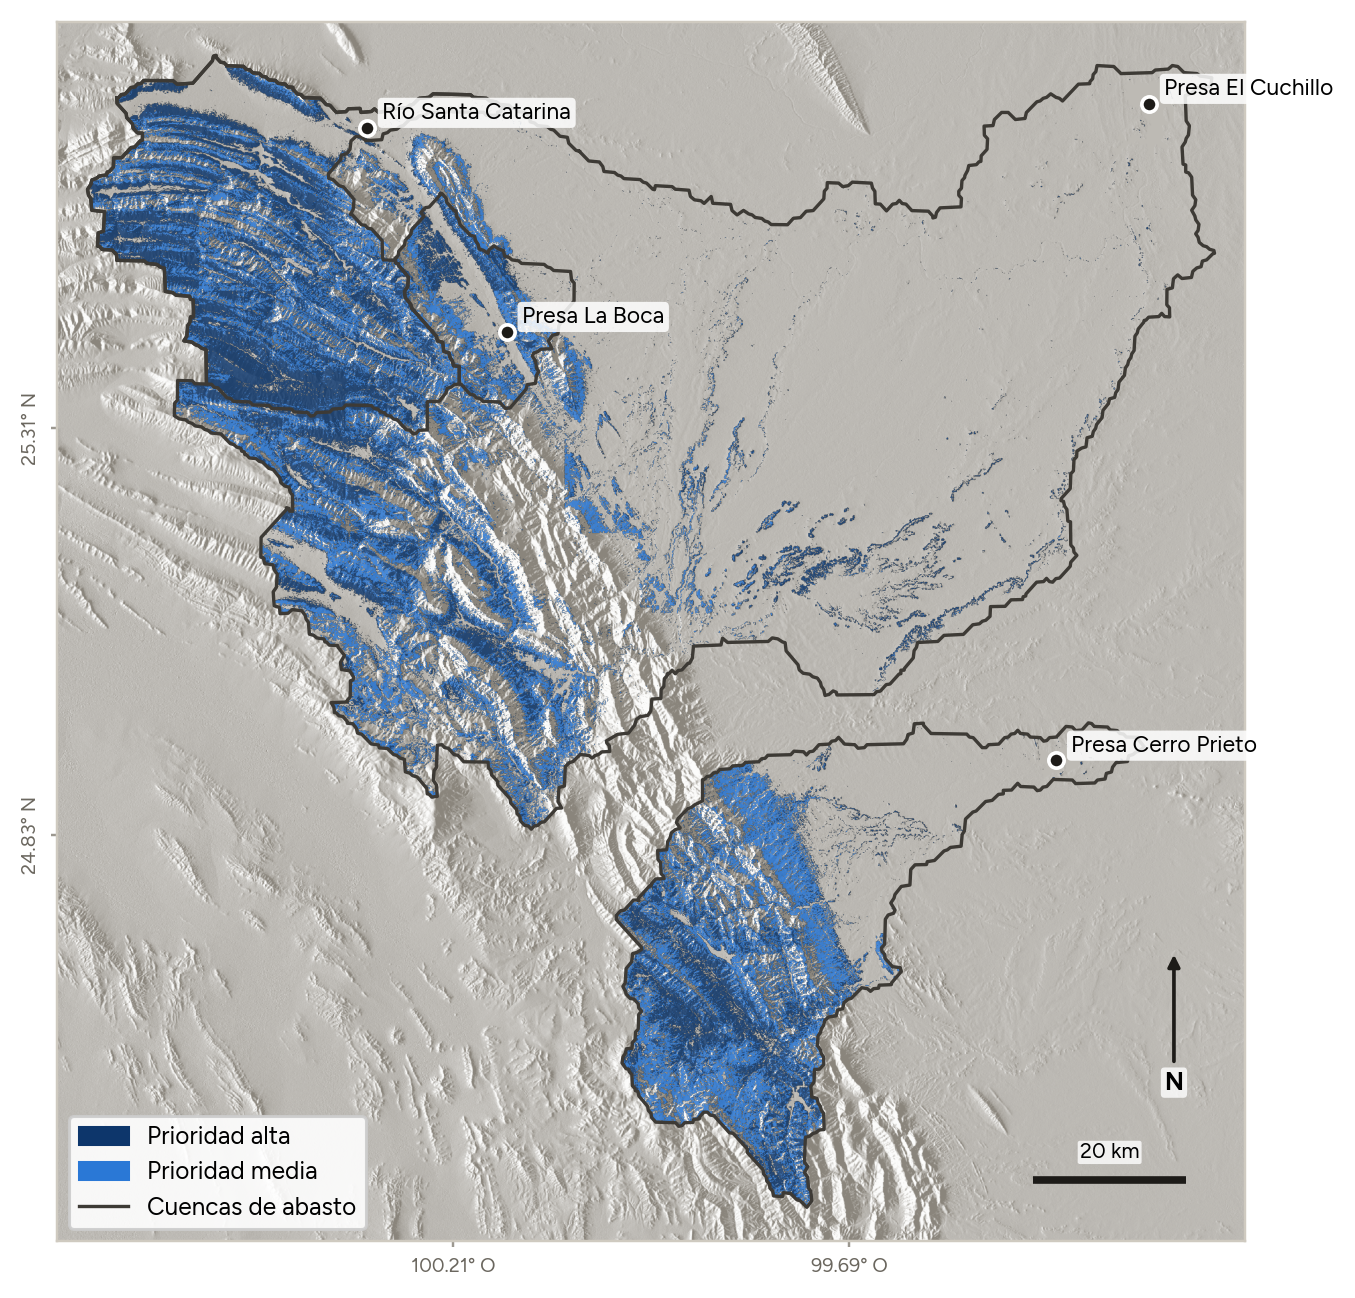
\includegraphics[width=\linewidth,height=0.72\textheight,keepaspectratio]{figuras/m1_cuencas.png}
\end{column}
\begin{column}{0.38\textwidth}
\cifra{«alta» ha}{de prioridad alta en laderas de 8° o más}
\vspace{0.3cm}

\cifra{«sc_alta» ha}{en la cuenca del Santa Catarina}
\vspace{0.3cm}

\cifra{«robusta_pct»}{robustas: no dependen de cómo se ponderen los criterios}
\nota{La conexión con el abasto se puntúa por la ganancia neta esperada de cada fuente: Santa Catarina 1, presas 0.5, resto de El Cuchillo 0.3.}
\end{column}
\end{columns}
\end{frame}

\begin{frame}{Las obras no desvían el agua: la retienen para que se infiltre}
\begin{columns}[T]
\begin{column}{0.5\textwidth}
\begin{itemize}
  \item 3,000 ha retienen unos \textbf{«max_ls» L/s de agua bruta} (intervalo de 90\%: «mc_p5» a «mc_p95» L/s).
  \item El agua retenida sigue por el subsuelo dentro de la misma cuenca: una parte se evapotranspira, otra recarga el acuífero o llega a la presa como flujo base.
  \item Sin obras, parte de esa agua habría llegado a la presa de todos modos.
\end{itemize}
\clave{Ganancia neta por m³ retenido:\quad $G=(1-e)\,\phi-\tau$\\[2pt]
{\scriptsize $e$: evapotranspiración · $\phi$: fracción que llega a la fuente · $\tau$: lo que ya llegaba sin obras}}
\end{column}
\begin{column}{0.48\textwidth}
\centering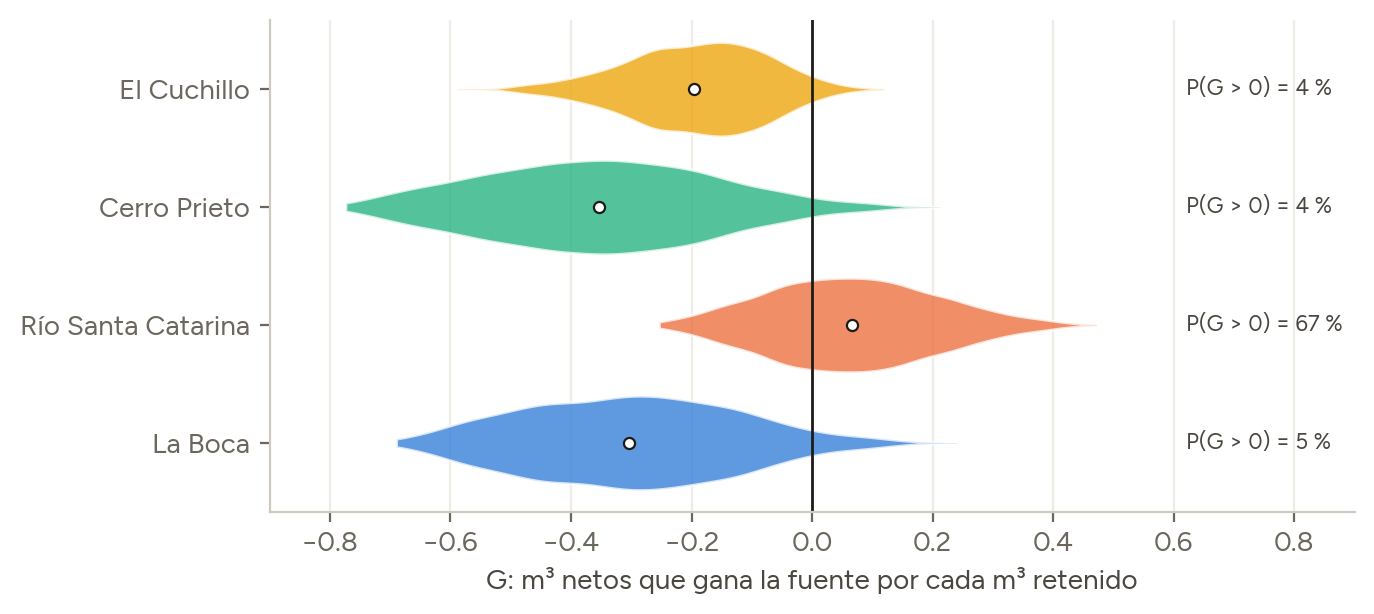
\includegraphics[width=\linewidth]{figuras/g14_destino.png}
\nota{«fate_n» escenarios de Monte Carlo; la evapotranspiración se acota con MODIS.}
\end{column}
\end{columns}
\end{frame}

\begin{frame}{Sólo el Santa Catarina gana agua neta}
\begin{columns}[T]
\begin{column}{0.47\textwidth}
\centering\small
\begin{tabular}{lrr}
\toprule
Fuente & $G$ medio & P($G>0$) \\
\midrule
Santa Catarina (acuífero) & «g_sc» & «pg_sc» \\
La Boca & «g_lb» & «pg_lb» \\
Cerro Prieto & «g_cp» & «pg_cp» \\
El Cuchillo & «g_ec» & «pg_ec» \\
\bottomrule
\end{tabular}
\vspace{0.4cm}

\begin{itemize}
  \item En el Santa Catarina, el escurrimiento de tormenta cruza la ciudad y se pierde: infiltrarlo en la sierra es \textbf{recarga nueva} para los pozos de SADM.
  \item En las presas, lo retenido ya llegaba al embalse: la retención \textbf{probablemente reduce} el agua que les llega.
\end{itemize}
\end{column}
\begin{column}{0.47\textwidth}
\centering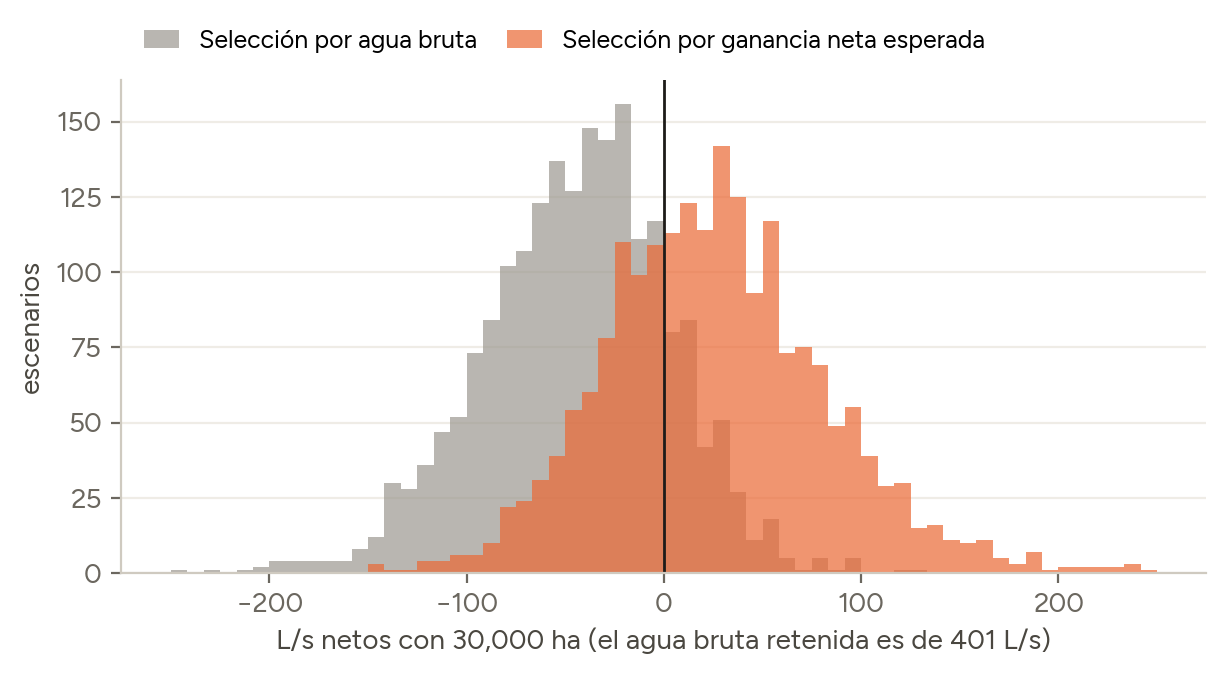
\includegraphics[width=\linewidth]{figuras/g15_neto.png}
\nota{30,000 ha seleccionadas por ganancia neta: unos «n30n_mean» L/s netos en promedio, con probabilidad «n30n_pp» de ser positivos.}
\end{column}
\end{columns}
\end{frame}

\begin{frame}{Frente a 2022, la restauración suma poco}
\begin{columns}[T]
\begin{column}{0.58\textwidth}
\centering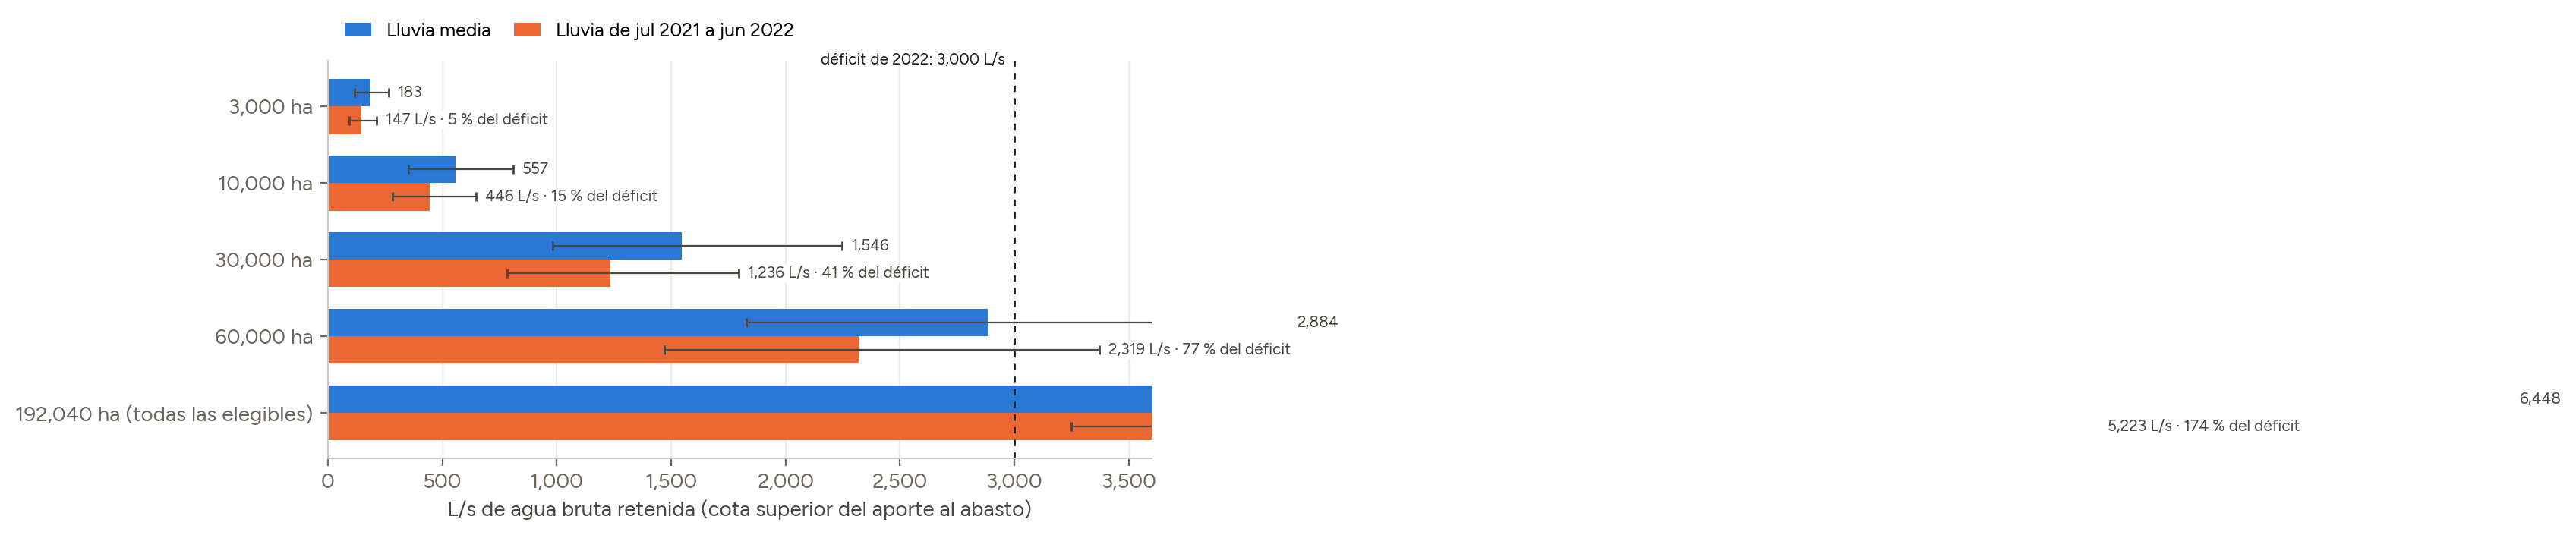
\includegraphics[width=\linewidth]{figuras/g13_abasto.png}
\end{column}
\begin{column}{0.4\textwidth}
\cifra{«ab30_pct»}{del déficit de 2022 con 30,000 ha, aun en agua bruta}
\vspace{0.3cm}

\cifra{«aball_pct»}{con las «ab_all_ha» ha elegibles (límite teórico)}
\vspace{0.3cm}

\cifra{«aq_def_pct_c» a «aq_def_pct_u»}{del déficit del acuífero Campo Buenos Aires (ganancia neta, 30,000 ha)}
\nota{La restauración no habría evitado la crisis: es una fuente complementaria.}
\end{column}
\end{columns}
\end{frame}

\begin{frame}{En las presas, el beneficio es el suelo, no el volumen}
\begin{columns}[T]
\begin{column}{0.5\textwidth}
\begin{itemize}
  \item Con la RUSLE, 30,000 ha en Cerro Prieto evitarían que lleguen unos \textbf{«sed30_50» hm³ de sedimento en 50 años}, del orden de «sed30_pct» de la capacidad de la presa.
  \item Pero reducirían el agua que le llega en unos \textbf{«sed30_wabs» hm³ por año}.
  \item En las cuencas de las presas, las obras se justifican por la conservación del suelo, la vida útil del embalse y la atenuación de avenidas.
\end{itemize}
\end{column}
\begin{column}{0.46\textwidth}
\centering
\cifra{«sed30_50» hm³}{de azolve evitado en 50 años}
\vspace{0.5cm}

\cifra{−«sed30_wabs» hm³/año}{de agua que deja de llegar a Cerro Prieto}
\end{column}
\end{columns}
\end{frame}

\begin{frame}{Como fuente de agua, la restauración es cara}
\begin{columns}[T]
\begin{column}{0.5\textwidth}
\begin{itemize}
  \item Costo: 25,000 a 50,000 pesos por hectárea (tope de CONAFOR para restauración forestal, 2026).
  \item Por L/s bruto: de «cb30_lo» a «cb30_hi» millones de pesos, del orden del acueducto El Cuchillo II.
  \item Por \textbf{L/s neto}: unos \textbf{«cn30» millones de pesos}, más de diez veces más.
  \item Probabilidad de que resulte más barata que El Cuchillo II por L/s: «cp30».
\end{itemize}
\nota{Sólo costo de capital; no incluye el bombeo ni la operación del acueducto, ni los beneficios distintos del agua.}
\end{column}
\begin{column}{0.46\textwidth}
\centering
\cifra{«cn30» M\$}{por L/s neto con restauración}
\vspace{0.5cm}

\cifra{2.9 M\$}{por L/s con El Cuchillo II (14,680 M\$ por 5,000 L/s)}
\end{column}
\end{columns}
\end{frame}

\begin{frame}{Dónde y cómo construir}
\begin{columns}[T]
\begin{column}{0.5\textwidth}
\centering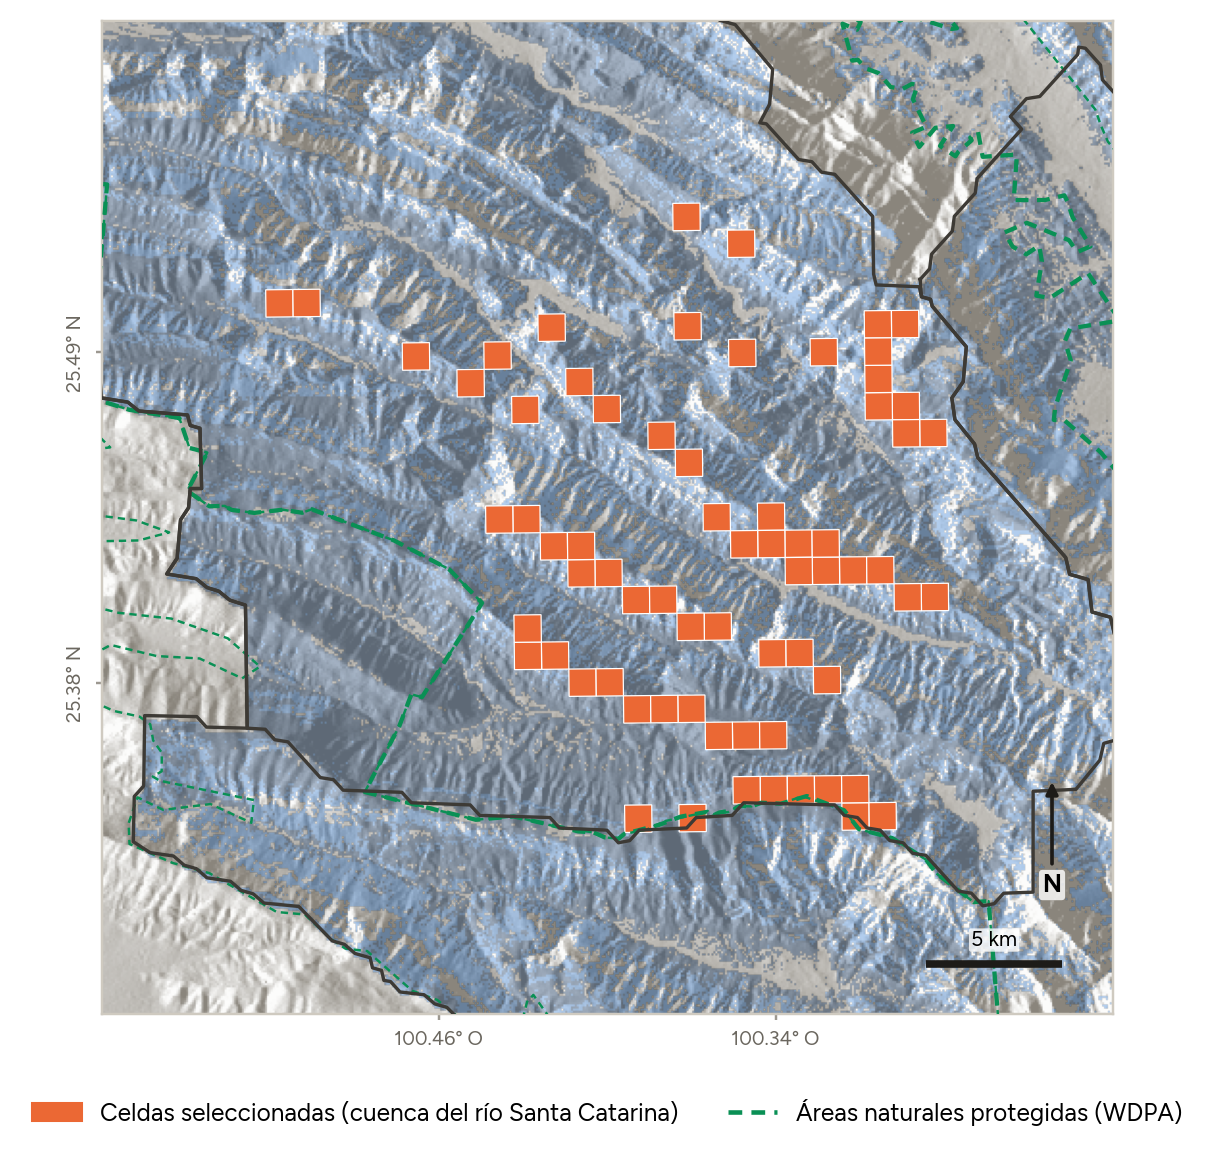
\includegraphics[width=\linewidth,height=0.66\textheight,keepaspectratio]{figuras/m2_optimizacion.png}
\end{column}
\begin{column}{0.48\textwidth}
\begin{itemize}
  \item Las celdas óptimas por ganancia neta están todas en el Santa Catarina; \textbf{«anp_cumbres3» de 3,000 ha} están en el Parque Nacional Cumbres de Monterrey: se requiere autorización de la CONANP.
  \item Ocho sitios sugeridos, separados al menos 3 km, con barreras trazadas por MCMF.
  \item En tormentas grandes manda la \textbf{capacidad} de las obras: 1,500 m de barreras retienen «ret5» de una tormenta de 5 mm y sólo «ret40» de una de 40 mm.
\end{itemize}
\end{column}
\end{columns}
\end{frame}

\begin{frame}{Vegetación: sólo especies del tipo de vegetación de cada ladera}
\footnotesize
\begin{tabularx}{\linewidth}{>{\raggedright\arraybackslash}p{3.4cm}>{\raggedright\arraybackslash}X>{\raggedright\arraybackslash}p{4.2cm}}
\toprule
Tipo de vegetación (INEGI) & Especies de referencia & Obra \\
\midrule
Matorral submontano & \emph{Acacia amentacea, Zanthoxylum fagara, Leucophyllum frutescens, Cordia boissieri, Helietta parvifolia} & Material vegetal muerto; arbustos ladera arriba \\
Matorral desértico & \emph{Agave lecheguilla, Larrea tridentata, Koeberlinia spinosa, Fouquieria splendens} & Piedra acomodada con lechuguilla \\
Bosque de encino & \emph{Quercus canbyi, Q. glaucoides, Q. laceyi, Juniperus, Arbutus xalapensis} & Zanja-bordo con encinos y enebros \\
Bosque de pino-encino & \emph{Pinus pseudostrobus, Q. rysophylla, Q. canbyi, Juniperus flaccida} & Material vegetal muerto y regeneración natural \\
Oyamel y ayarín & Requiere inventario de campo (posible NOM-059) & Sólo conservación de suelo \\
\bottomrule
\end{tabularx}
\nota{Material de procedencia local y densidad moderada: una cobertura densa eleva la evapotranspiración y reduce la ganancia neta. Inventarios: Alanís-Rodríguez et al. (2015a, b), Jiménez Pérez et al. (2013), Ramírez-Lozano et al. (2013).}
\end{frame}

\begin{frame}{Qué tan sólidos son los resultados}
\begin{itemize}
  \item \textbf{Calibración:} contra el escurrimiento natural oficial de Cerro Prieto (CONAGUA), el modelo sobrestima el escurrimiento; calibrado, el agua bruta y la neta bajan alrededor de «cal_drop», sin cambiar la probabilidad de ganancia positiva.
  \item \textbf{Acuífero:} la recarga adicional en el Santa Catarina es «aq_net_pct» de la recarga natural del acuífero Campo Buenos Aires: físicamente plausible.
  \item \textbf{Sequía:} con la lluvia de 2021 a 2022 se conserva «dr_pct» del agua bruta y «dr_overlap» de los sitios.
  \item \textbf{Clima 2041 a 2070:} la frecuencia de un año tan seco como 2021 a 2022 sería de «clima_f245» (SSP2-4.5) y «clima_f585» (SSP5-8.5), con mucha dispersión entre modelos.
  \item \textbf{Lo más incierto:} la evapotranspiración del agua infiltrada y la fracción del escurrimiento que ya llega a las presas. No están calibradas.
\end{itemize}
\end{frame}

\begin{frame}{Recomendaciones}
\begin{enumerate}
  \item \textbf{Restaurar primero las laderas del Santa Catarina}, donde el abasto sí gana agua, con autorización de la CONANP dentro del Parque Nacional Cumbres de Monterrey.
  \item \textbf{En las cuencas de las presas}, restaurar por el suelo, la vegetación y la vida útil de los embalses, sin esperar más agua.
  \item \textbf{Acompañar cada obra} sólo con especies nativas de su tipo de vegetación, de procedencia local y a densidad moderada.
  \item \textbf{Medir antes de escalar:} microcuencas pareadas con vertedores, humedad del suelo y piezómetros en los ocho sitios (unos 16 pares para detectar una diferencia de 50\%), más pares en Cerro Prieto.
  \item \textbf{Presentar la restauración como complemento}, no como sustituto de otras fuentes de abasto.
\end{enumerate}
\end{frame}

\begin{frame}[plain]
\vspace{1.5cm}
\centering
{\color{naranja}\Large\bfseries Gracias\par}
\vspace{0.6cm}
{\small Informe completo, aplicación y código:\par}
{\small\color{verde}\url{https://github.com/pcruiher08/InflitracionAguaNuevoLeon}\par}
{\small\color{verde}\url{https://pcruiher08.github.io/InflitracionAguaNuevoLeon/}\par}
\vspace{0.8cm}
{\scriptsize\color{gris}M.Sc. Pablo César Ruíz Hernández · B.Sc. David Martin Oliva Zavala · Jesus Zaddkiel Martinez Alor\par}
\end{frame}

\end{document}
